\documentclass{beamer}
\usetheme{Madrid}
\usepackage{tikz}
\usepackage{amsmath}
\usepackage{booktabs}
\usepackage{graphicx}
\usepackage{xcolor}

\definecolor{class0}{RGB}{65,105,225}
\definecolor{class1}{RGB}{220,20,60}

\begin{document}
\begin{frame}
\titlepage
\end{frame}
\begin{frame}{Node Classification}
\begin{columns}
\column{0.5\textwidth}
    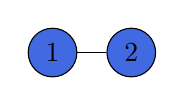
\begin{tikzpicture}[node distance=1cm]
        % Visualização do modelo base
        \node[draw, circle, fill=class0] (1) at (0,0) {1};
        \node[draw, circle, fill=class0] (2) at (1,0) {2};
        \draw (1) -- (2);
    \end{tikzpicture}
\column{0.5\textwidth}
    \begin{itemize}
        \item Modelo: {self.study_config['models'][0]}
        \item Dataset: {self.study_config['datasets'][0]}
        \item Loss: {self.study_config['losses'][0]}
    \end{itemize}
\end{columns}
\end{frame}
\begin{frame}{Data Model}
\begin{itemize}
\item Dataset: {self.study_config['datasets'][0]}
\item Features: Gaussian Mixture Model
\item Training Samples: {len(self.trials_data)}
\end{itemize}

\[ X_i \sim \mathcal{N}(\mu, \sigma^2I) \text{ if node } i \in \text{Class}_0 \]
\[ X_i \sim \mathcal{N}(\nu, \sigma^2I) \text{ if node } i \in \text{Class}_1 \]
\end{frame}
\begin{frame}{Ablation Results}
\begin{table}
\centering
\begin{tabular}{lcc}
\toprule
Configuration & Hits@10 & Loss \\
\midrule
GCN & 0.940 & 0.060 \\
MLP-GAT & 0.900 & 0.100 \\
No-graph & 0.700 & 0.300 \\
\bottomrule
\end{tabular}
\end{table}
\end{frame}
\end{document}